\documentclass[11pt]{article}
\title{\textbf{Horns unit}}
\author{https://github.com/heptagons/meccano/units/horns}
\date{}

\usepackage{../../meccano}
\usepackage{tikz}
\usetikzlibrary{calc}

\begin{document}

\maketitle
\begin{abstract}
Horns unit is a group of seven meccano\meccanoref strips intended to build polygons.
\end{abstract}

\begin{figure}[h]
\centering
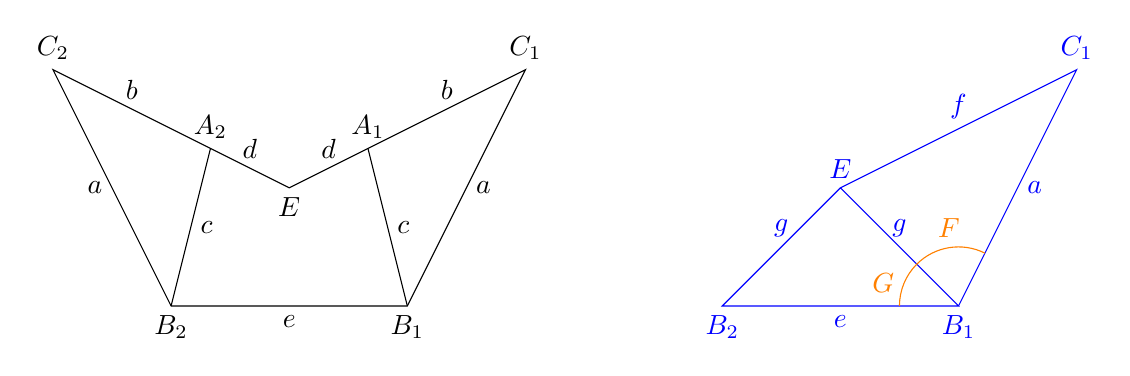
\begin{tikzpicture}
 \begin{scope}[scale=0.5]
  \draw[black] (0,0)
  -- node[below] {$e$} ++(6,0) node[below] {$B_1$}
  -- node[below,right] {$a$} ++(3,6) node[above] {$C_1$}
  -- node[above] {$b$} ++(-4,-2) node[above] {$A_1$}
  -- node[above] {$d$} ++(-2,-1) node[below] {$E$}
  -- node[above] {$d$} ++(-2,1) node[above] {$A_2$}
  -- node[above] {$b$} ++(-4,2) node[above] {$C_2$}
  -- node[below,left] {$a$} ++(3,-6) node[below] {$B_2$}
  -- cycle;
  \draw[black] (6,0) --++ (-1,4) node[midway,right] {$c$};
  \draw[black] (0,0) --++ (+1,4) node[midway,right] {$c$};

  \draw[blue] (20,0)
  -- node[below,right] {$a$} ++(3,6) node[above] {$C_1$}
  -- node[above] {$f$} ++(-6,-3) node[above] {$E$}
  -- node[above] {$g$} ++(-3,-3) node[below] {$B_2$}
  -- node[below] {$e$} ++(6,0) node[below] {$B_1$}
  -- node[above] {$g$} ++(-3,+3);
  
  \draw[orange] (20,0)+(-1.5,0) 
   arc (180:135:1.5) node[midway,above,left] {$G$}
   arc (135:atan(2):1.5) node[midway,above] {$F$};
 \end{scope}

\end{tikzpicture}
\caption{The \textbf{horn unit} has seven strips: Two of length $a$, two of length $b+d$,
two of length $c$ and one of length $e$.
We expect to build polygons with internal angle $C_1B_1B_2$
and perimeter including segments $a,e,a$.}
\label{fig:horns}
\end{figure}

\section{Algebra}
From figure \ref{fig:horns} we start with triangle $\triangle{A_1B_1C1}$.
At vertex $A_1$ we have angle $A$ and the supplement $A'$:
\begin{align}
A &\equiv \angle{B_1A_1C_1}\\
\cos{A} &= \frac{b^2 + c^2 - a^2}{2bc} &\text{if and only if } a < b+c\\
A' &\equiv \angle{EA_1B_1} = \pi - A\\
\cos{A'} &= \cos{(\pi-A)} = -\cos{A} = \frac{- b^2 - c^2 + a^2}{2bc}
\end{align}

We define $f=b+d$ and $g \equiv \overline{EB_1}$ and with the law of cosines we have:
\begin{align}
f &\equiv b + d\\
g^2 &= c^2 + d^2 - 2cd\cos{A'}\\
 &= c^2 + d^2 - (2cd)\frac{-b^2 - c^2 + a^2}{2bc}\\
 &= \frac{bc^2 + bd^2 + b^2d + c^2d - a^2d}{b}\\
 &= \frac{(b+d)(bd+c^2) - a^2d }{b}\\
 &= \frac{(bd+c^2)f - a^2d }{b}\\
 &\equiv \frac{h}{b} &\text{if and only if } -b < h < b\\
\end{align}

We sum the angles $F$ and $G$ to get:
\begin{align}
F &\equiv \angle{C_1B1E}\\
\cos{F} &= \frac{a^2 + g^2 - f^2}{2ag}\\
G &\equiv \angle{B_2B_1E}\\
\cos{G} &= \frac{e}{2g}\\
F+G &\equiv \angle{B_2B_1C_1}\\
\cos{(F+G)} &= \cos{F}\cos{G} - \sin{F}\sin{G}\\
\end{align}

We calculate cosines part and replacing $g^2$ with $h/b$ first in the denominator
and finally in the numerator:
\begin{align}
\cos{F}\cos{G} &= \frac{a^2 + g^2 - f^2}{2ag} \times \frac{e}{2g}\\
 &= \frac{e(a^2 + g^2 - f^2)e}{4ag^2}\\
 &= \frac{e(a^2b + bg^2 - bf^2)}{4ah}\\
 &= \frac{e(a^2b + h - bf^2)}{4ah}
\end{align}

We calculate the sines part squared. Replace $g^2$ with $h/b$ first in the denominator:
\begin{align}
(\sin{F}\sin{G})^2 &= (1 - cos^2{F})(1 - cos^2{G})\\
 &= 1 - cos^2{F} - cos^2{G} + cos^2{F}\cos^2{G}\\
 &= 1 - \frac{(a^2 + g^2 - f^2)^2}{4a^2g^2} - \frac{e^2}{4g^2} + (\cos{F}\cos{G})^2\\
 &= 1 - \frac{b(a^2 + g^2 - f^2)^2}{4a^2h} - \frac{be^2}{4h} + \frac{e^2(a^2b + h - bf^2)^2}{16a^2h^2}\\
 &= \frac{16a^2h^2}{16a^2h^2} 
 - \frac{4bh(a^2 + g^2 - f^2)^2}{16a^2h^2} 
 - \frac{4a^2be^2h}{16a^2h^2} 
 + \frac{e^2(a^2b + h - bf^2)^2}{16a^2h^2}\\
\end{align}





\end{document}
